The purpose of this thesis was to categorize the dark web and visualize the result. In order to do that, the dark web had been scraped and the acquired pages had been stored in an ElasticSearch database. This was done as part of a bachelor's thesis which was being completed at the same time as this thesis. In order to retrieve the data from the database and do various operations on them, a back-end (BE) needed to be created. One of the operations was the categorization of the acquired pages. For that, an appropriate topic modeling approach was required. We chose to adopt the Latent Dirichlet Allocation (LDA). To visualize the output a graph was used. However, the data set is rather sizable and to be able to provide the user with useful information, not all pages can be displayed at once. Therefore a proper way to divide the graph into several subgraphs had to be found. We decided to use the well known Louvain algorithm (LA). To display the graph in a comprehensible manner a front-end (FE) was created.

In this chapter we will describe LDA,  which is the method used to categorize the scraped pages. Next we will talk about why it is necessary to divide immense numbers of data into clusters in order to display them as a graph. And lastly, we will detail communities and LA, the algorithm for dividing pages into communities. 

\section{Web graph} \label{webGraph}
We display our data as a graph. More precisely a web graph \cite{the_web_graph_overview}. A web graph is a graph representation of the web where nodes are portrayals of the pages and edges depict links between the pages. Web graphs tend to be built from an enormous amount of data. As such, they can  be advertised in various ways. One of the visualizations is shown in figure  \ref{hugeWebGraphFireworks}. 
\begin{figure}[ht!]
  \centering
  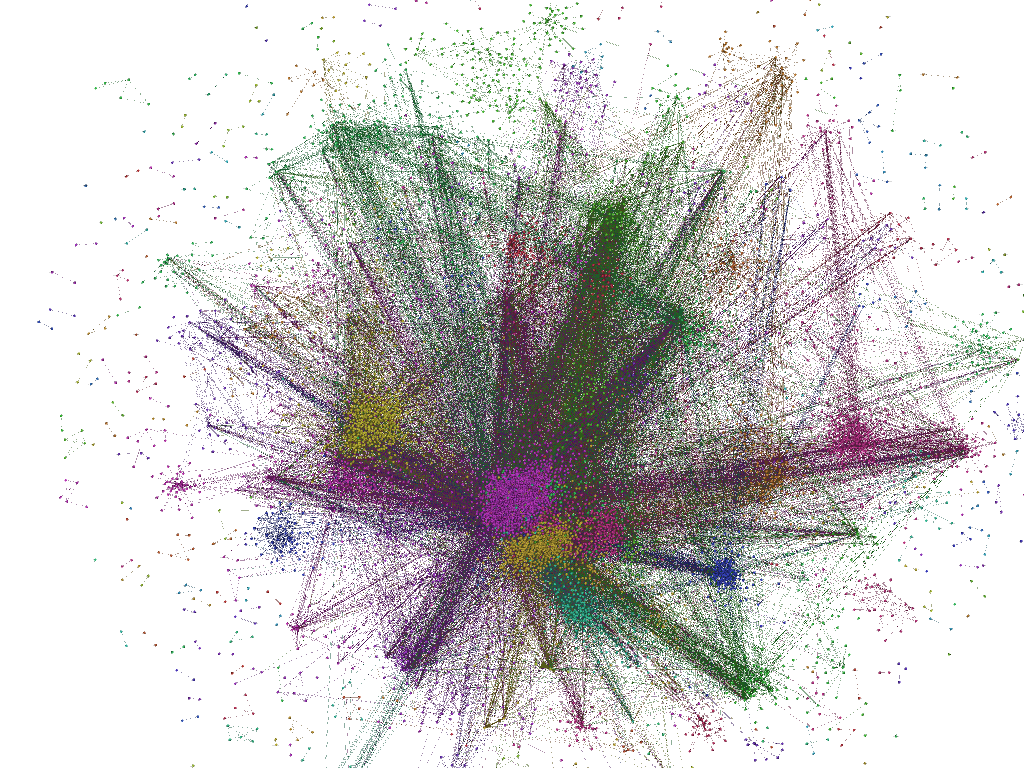
\includegraphics[width=\textwidth]{Images/hugeWebGraphFireworks.png}
  \caption{Web graph by Citeo.}
  \label{hugeWebGraphFireworks}
\end{figure} 
The web graph depicted displays all its data at once without any labels or details. The result might be useful for viewing the internet as a whole but for our purposes was insufficient since a user has had to be able to view the relationships between nodes in more detail along with information about the pages. The web graph needed to be composed of a significant smaller amount of nodes so that the view port was not too cluttered and the sought knowledge could be obtained with as little hindrances as possible. Because the majority of the nodes in the graph were not isolated \footnote{An isolated node is a node with zero incoming and outgoing edges.} and were in fact part of a single connected component it was possible to partition the graph based on the density of its nodes, the so called communities.

\subsection{Community structure}
If a graph can be partitioned into several subgraphs so that nodes from one subgraph are internally connected densely and are connected scarcely to nodes from other subgraphs, we can claim it has a  community structure with each subgraph as a community \cite{communitiesOverview}. Each community can be portrayed as a meta node of the graph and so possibly reduce the number of nodes in the graph dramatically. The quality of such a partition can be measured using modularity. \cite{modularityOverview} \begin{quotation}  For a candidate partition of the vertices into clusters, the modularity is defined to be the portion of the edge connections within the same cluster minus the expected portion if the connections were distributed randomly \end{quotation} \cite{modularityDefinition}

\section{Louvain algorithm} \label{louvainAlgorithm}
A profoundly used algorithm for finding communities in graphs is LA \cite{louvainAlgorithm}. It is a greedy algorithm which maximizes modularity locally. Each node is assigned a community. Afterwards the node is taken out of its community and randomly appointed to the communities of its neighbours. After the node visited communities of all its neighbours it is left in the one with the maximum modularity value, which can also result in it remaining in its original community. Next, the algorithm runs on the newly gathered communities and tries to assign each whole community to its neighbouring communities in a similar manner. This is repeated until the modularity cannot be improved further.

LA is favoured for its simplicity, speed and accuracy. Since its discovery, in 2008, it was possible to detect communities in graphs with billions of nodes in a relatively timely manner. LA was compared to other algorithms for community detection, namely the algorithm of Wakita andTsurumi \cite{wakitaAndToshiyuki}, of Pons and Latapy \cite{ponsAndLatapy}, and of Clauset, Newman and Moore \cite{CNM} on graphs of sizes varying between 34 nodes and 77 edges to as much as 118 million nodes and 1 billion edges. The difference between the computing times of the previously stated algorithms grows with the size of the graphs and favours LA. In fact, it took 152 minutes for LA to detect the communities of the greatest graph whereas the computation time of the other algorithms was more than 24 hours. In terms of precision, LA was also the most precise one with slightly better modularities.

